%% Seminar deck: Microstructure-Efficient Estimation of Sovereign Yield
%% Curves in Less-Liquid Markets (SNDE, 2026, doi:10.1515/snde-2026-0057).
%% Built from the published article, not from the WP#53 deck. House style.
\documentclass[aspectratio=169,11pt]{beamer}
\usepackage{beamerthemeyc}
\usepackage{booktabs}
\usepackage{multirow}
\renewcommand{\deckfootertitle}{Dec · Microstructure-efficient sovereign yield curves · SNDE 2026 · doi:10.1515/snde-2026-0057}

\newcommand{\GM}{\mathrm{GM}}
\newcommand{\HS}{\mathrm{HS}}
\newcommand{\out}{\mathrm{out}}

\begin{document}

% 1 — title --------------------------------------------------------------------
\begin{frame}[plain]
  \vspace{2mm}
  {\ttfamily\scriptsize\color{ycmuted}SEMINAR DECK · YIELDCARTOGRAPHY.COM}\\[-0.3em]
  {\color{ycrule}\rule{\textwidth}{0.5pt}}
  \vspace{4mm}

  {\fontsize{19}{23}\selectfont\bfseries\color{ycink}Microstructure-efficient estimation of\\sovereign yield curves in less-liquid markets.\par}
  \vspace{2mm}
  {\normalsize\color{ycmuted}Glosten-Milgrom and Ho-Stoll foundations for liquidity-weighted NSS fitting,\\with asymptotics, identification and a 21-year Polish bond panel.\par}
  \vspace{5mm}
  {\small\bfseries Marcin Dec\par}
  {\footnotesize\color{ycmuted}Kozminski University \& FAME|GRAPE, Warsaw\par}
  \vspace{3mm}
  {\ttfamily\scriptsize\color{ycaccent}Studies in Nonlinear Dynamics \& Econometrics · online 7 October 2026 · open access (CC-BY)\\doi:10.1515/snde-2026-0057\par}
  \vfill
  \raisebox{-1mm}{
\includegraphics[height=6mm]{kozminski_logo.png}}\hspace{5mm}
  \raisebox{-1mm}{
\includegraphics[height=6mm]{grape_logo.png}}\hspace{5mm}
  \raisebox{-1mm}{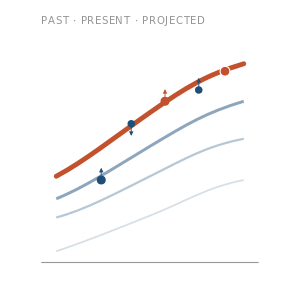
\includegraphics[height=6mm]{yc_logo.png}}
  \hfill{\ttfamily\scriptsize\color{ycmuted}NCN Preludium UMO-2020/37/N/HS4/02202}
\end{frame}

% 2 — motivation ---------------------------------------------------------------
\begin{frame}{Motivation and question}
  \kicker{From practitioner patches to a derived estimator}
  \begin{itemize}
    \item In a less-liquid sovereign market the fixing on a rarely traded
          bond is a far noisier signal than one on a benchmark issue:
          observation noise is strongly heteroskedastic across bonds.
    \item Practice has accumulated patches without foundations: turnover or
          outstanding weights tuned by hand, a $\tau_1$ floor, a curvature
          ridge, a residual-maturity filter.
    \item The paper derives the efficient weight matrix for the
          Nelson-Siegel-Svensson fit from two dealer-market models, proves
          consistency, normality and Aitken efficiency, and turns the
          patches into corollaries of a rank analysis.
    \item Validated on a Monte Carlo grid and on 5{,}319 Polish daily
          cross-sections, 2005 to 2026.
  \end{itemize}
\end{frame}

% 3 — estimator ----------------------------------------------------------------
\begin{frame}{The LW-NSS estimator}
  \kicker{Weighted nonlinear least squares in yield space}
  \small The zero curve follows Svensson (1994):
  \[ y(\tau;\theta) = \beta_0
     + \beta_1 \tfrac{1-e^{-\tau/\tau_1}}{\tau/\tau_1}
     + \beta_2 \Big( \tfrac{1-e^{-\tau/\tau_1}}{\tau/\tau_1} - e^{-\tau/\tau_1} \Big)
     + \beta_3 \Big( \tfrac{1-e^{-\tau/\tau_2}}{\tau/\tau_2} - e^{-\tau/\tau_2} \Big) \]
  and the LW-NSS estimator solves, per settlement date,
  \[ \hat\theta_{\mathrm{LW}} \;=\; \arg\min_{\theta\in\Theta} \sum_{i=1}^{N}
     w_{y,i}\, \big( y_i - \hat y_i(\theta) \big)^2 . \]
  \begin{itemize}
    \item Equal weights (Diebold-Li, G\"urkaynak-Sack-Wright), duration
          weights and ad-hoc turnover blends coexist in practice. The open
          question is which $w_{y,i}$ a microstructure model actually implies.
  \end{itemize}
\end{frame}

% 4 — GM channel ---------------------------------------------------------------
\begin{frame}{Channel one: adverse selection (Glosten-Milgrom)}
  \kicker{A yield-space dealer problem delivers the turnover weight}
  \begin{itemize}
    \item The fixing on bond $i$ is the dealer's posterior mean of the
          fundamental yield after a Glosten-Milgrom quoting process run in
          the yield coordinate. In the active-trading regime the posterior
          variance is
          \[ \sigma_{y,i}^2 \;\approx\; \frac{\kappa}{\mu_i}, \]
          with $\mu_i$ the bond's turnover intensity. Duration does not enter
          the noise of a yield quote, it is only the price-to-yield Jacobian.
    \item \textbf{Theorem (optimal GM weight).} The efficient GLS weight is
          the inverse noise variance, $w_{y,i} = \mu_i/\kappa$: the
          turnover-weighted fit is minimum-variance unbiased within weighted
          NLS on yield residuals (Aitken).
  \end{itemize}
\end{frame}

% 5 — HS channel + hybrid ------------------------------------------------------
\begin{frame}{Channel two and the hybrid: inventory risk (Ho-Stoll)}
  \kicker{One dominance ratio governs the blend}
  \begin{itemize}
    \item A complementary Ho-Stoll inventory channel delivers
          $w_{y,i,\HS} = \out_i/\kappa_{\HS}$, with $\out_i$ the outstanding
          amount. With both channels active and additive,
          \[ \sigma_{y,i}^2 \;=\; \frac{\kappa_{\GM}}{\mu_i}
             + \frac{\kappa_{\HS}}{\out_i}
             \qquad\Longrightarrow\qquad
             w_{y,i,\mathrm{hybrid}}
             \;=\; \frac{\mu_i\,\out_i}{\kappa_{\HS}\,\mu_i + \kappa_{\GM}\,\out_i}. \]
    \item The blend is governed by a single dominance ratio
          $\rho = \kappa_{\HS}/\kappa_{\GM}$, not separately identified at a
          single date but identifiable from a panel of dates by minimising
          leave-one-out yield-prediction error.
    \item The linear turnover-outstanding blend used heuristically in
          less-liquid markets is the first-order arithmetic-mean
          approximation to this harmonic-mean hybrid.
  \end{itemize}
\end{frame}

% 6 — asymptotics --------------------------------------------------------------
\begin{frame}{Asymptotic theory}
  \kicker{M-estimation under conditional heteroskedasticity}
  \begin{itemize}
    \item The LW-NSS fit is a nonlinear M-estimator at fixed settlement date
          with $N\to\infty$, a thought experiment about a denser market that
          characterises the local behaviour of $\hat\theta$ on the observed
          panel.
    \item Consistency and asymptotic normality hold with sandwich variance
          \[ \sqrt{N}\,(\hat\theta - \theta_0)
             \;\xrightarrow{d}\;
             N\!\big(0,\; Q^{-1}\,\Omega\, Q^{-1}\big),
             \qquad Q = \mathrm{plim}\,\tfrac{1}{N} J' W J, \]
          collapsing to $Q^{-1}$ (up to scale) under correct specification.
    \item \textbf{Aitken efficiency.} The inverse-variance weight attains the
          Cram\'er-Rao style bound within the weighted NLS class, so any
          misspecified weight (equal weights included) is weakly less
          efficient, uniformly across GM, HS and hybrid. A robust variance
          estimator covers the misspecified case.
  \end{itemize}
\end{frame}

% 7 — identification -----------------------------------------------------------
\begin{frame}{Identification under sparse panels}
  \kicker{A four-band coverage condition on the maturity grid}
  \begin{itemize}
    \item The Svensson loadings peak at $\tau \approx 1.7933\,\tau_1$ and
          $1.7933\,\tau_2$, which pins a four-band partition of the maturity
          axis:
          \[ B_1 = [0,\tfrac{\tau_1}{2}], \quad
             B_2 = [\tfrac{\tau_1}{2}, 2\tau_1], \quad
             B_3 = [2\tau_1, \tfrac{\tau_2}{2}], \quad
             B_4 = [\tfrac{\tau_2}{2}, \infty). \]
    \item \textbf{Proposition.} The information matrix $\tfrac1N J'WJ$ is
          positive definite if and only if each band carries nonnegligible
          weight. Proof by Schur-complement partition into
          $(\beta_0,\beta_1,\beta_2,\tau_1)$ and $(\beta_3,\tau_2)$ blocks.
    \item \textbf{Corollaries.} When a band fails, a constrained fit fixing
          the corresponding decay at the boundary is consistent for the
          projection onto the restricted submanifold. The practitioner
          $\tau_1$ floor and the curvature ridge are exactly these
          constrained estimators.
  \end{itemize}
\end{frame}

% 8 — MC design ----------------------------------------------------------------
\begin{frame}{Monte Carlo design}
  \kicker{Controllable panels around the rank-condition boundary}
  \begin{itemize}
    \item Mid-cycle Svensson truth
          $\theta_0 = (0.04, -0.01, 0.02, 0.01, 1.5, 5.0)$, pricing errors
          calibrated so a typical bond has $\sigma_{y,i}\approx 8$ bp,
          matching the Polish panel scale. 250 replications per cell,
          multi-start Levenberg-Marquardt.
    \item Grid crosses panel size $N \in \{12, 18, 24, 36\}$, three sparsity
          regimes (dense, moderate gap, severe gap with two of the four bands
          undercovered, mimicking the 2008-2009 Polish panel), and three
          liquidity-heterogeneity regimes (homogeneous, Pareto 80/20,
          extreme Pareto 95/10).
    \item Three noise DGPs (pure GM, pure HS, hybrid) against four
          estimators: E1 equal weights, E2 turnover (GM), E3 outstanding
          (HS), E4 hybrid with grid-searched dominance ratio.
  \end{itemize}
\end{frame}

% 9 — MC results ---------------------------------------------------------------
\begin{frame}{Monte Carlo results}
  \kicker{Median integrated yield-curve MSE, basis points squared}
  \begin{center}
  \small
  \begin{tabular}{lcccc}
  \toprule
  DGP & E1 (equal) & E2 (GM) & E3 (HS) & E4 (hybrid) \\
  \midrule
  Pure GM noise     & 108.6 & \textbf{69.2} & 97.6 & 77.1 \\
  Pure HS noise     & 117.6 & 115.2 & \textbf{71.8} & 79.8 \\
  Hybrid GM+HS noise & 131.0 & 100.6 & 98.0 & \textbf{91.2} \\
  \bottomrule
  \end{tabular}
  \end{center}
  \vspace{2mm}
  \begin{itemize}
    \item Equal weighting is uniformly worst, 50 to 60 percent above the
          channel-matched alternative. The channel-matched estimator wins
          under its own DGP, and the hybrid trails the winner by under
          10 bp$^2$ everywhere while dominating under hybrid noise.
    \item The condition number of $J'WJ$ rises by a factor of about 50 from
          dense to severe-gap panels, validating the identification result.
  \end{itemize}
\end{frame}

% 10 — data --------------------------------------------------------------------
\begin{frame}{The Polish bond panel, 2005-2026}
  \kicker{BondSpot quote-driven primary-dealer venue}
  \begin{itemize}
    \item End-of-day fixings on 5{,}322 trading dates from 2005-01-03 to
          2026-04-21. On a typical date 17.4 bonds are listed, of which on
          average 15.1 enter the fit. Three thin dates are dropped, leaving
          5{,}319 daily cross-sections.
    \item Each bond carries a closing mid-price, a coupon-and-redemption
          schedule, a monthly turnover proxy and an outstanding face value,
          both disclosed by the Ministry of Finance.
    \item The minimum-residual-maturity filter (0.85 years before 2017-05-12,
          1.20 years thereafter) excludes bonds distorted by the Treasury
          switch-auction option.
    \item Headline tests run on 60 dates sampled uniformly across the panel.
          The term-premium exercise uses the full panel.
  \end{itemize}
\end{frame}

% 11 — empirical headline ------------------------------------------------------
\begin{frame}{Headline result: leave-one-out yield prediction}
  \kicker{LOO MAE in basis points, 60 sample dates}
  \begin{center}
  \small
  \begin{tabular}{lcccc}
  \toprule
  Statistic & E1 (equal) & E2 (GM) & E3 (HS) & E4 (hybrid) \\
  \midrule
  Median LOO MAE (bp)          & 9.34 & 8.60 & 9.42 & \textbf{8.37} \\
  Mean LOO MAE (bp)            & 9.23 & 8.82 & 9.14 & \textbf{8.72} \\
  75th-percentile LOO MAE (bp) & 12.61 & 11.99 & 12.60 & \textbf{11.99} \\
  Win rate vs E1 (\%)          & ref. & 75.0 & 50.0 & \textbf{78.3} \\
  \bottomrule
  \end{tabular}
  \end{center}
  \vspace{2mm}
  \begin{itemize}
    \item The empirical pattern reproduces the simulation: equal weighting is
          uniformly worst, the hybrid weight cuts the median error by about
          one basis point and beats equal weights on 78 percent of dates.
    \item Wilcoxon signed-rank test on per-date differences, one-sided:
          $W = 439$, $p = 0.0002$ for E2 vs E1 on $n = 60$ dates, with an
          equally significant rejection for the hybrid.
  \end{itemize}
\end{frame}

% 12 — regimes -----------------------------------------------------------------
\begin{frame}{When does the inventory channel matter?}
  \kicker{Regime-conditional split by the grid-best dominance ratio}
  \begin{center}
  \small
  \begin{tabular}{lcc}
  \toprule
  & GM-dominant ($n=40$) & HS-leaning ($n=20$) \\
  \midrule
  Median 2y zero yield (\%)   & 4.70 & 1.99 \\
  Median 10y zero yield (\%)  & 5.57 & 3.41 \\
  Median 10y$-$2y slope (bp)  & 83   & 120  \\
  Calendar concentration      & 2005-2011, 2017-2026 & 2012-2016 \\
  \bottomrule
  \end{tabular}
  \end{center}
  \vspace{2mm}
  \begin{itemize}
    \item On GM-dominant dates pure turnover weighting matches the hybrid
          (under 0.1 bp apart). On HS-leaning dates the hybrid beats pure GM
          by about 0.7 bp median LOO MAE, the entire empirical edge.
    \item The inventory channel activates when yields are low and the curve
          is steep (2012-2016), adverse selection dominates otherwise. The
          split is robust to the $\rho$ grid and the regime boundary.
  \end{itemize}
\end{frame}

% 13 — ACM downstream ----------------------------------------------------------
\begin{frame}{Downstream: ACM term premia inherit the wedge}
  \kicker{Same fitted histories, same ACM specification, only the weights differ}
  \begin{itemize}
    \item Every cross-section is refitted under the four schemes and passed
          through the same Adrian-Crump-Moench model ($K=5$ principal
          components, monthly resampling, daily projection).
    \item The 10-year term premium moves by 2.6 bp in median absolute
          difference between equal and hybrid weighting, 95th percentile
          8.5 bp, mean signed difference zero: the weighting changes the
          day-to-day path, not the level.
    \item The wedge is widest when the panel was thinnest (2005-2011, 95th
          percentile 13.3 bp) and narrowest after 2017. Pure GM and hybrid
          are nearly indistinguishable (0.6 bp median).
    \item The wedge is the same order as the curve-fitting gain itself, as an
          order-one pass-through from the long fitted yield into the premium
          predicts.
  \end{itemize}
\end{frame}

% 14 — takeaways ---------------------------------------------------------------
\begin{frame}{Takeaways}
  \kicker{Patches become corollaries}
  \begin{itemize}
    \item Turnover weighting is the information-matrix optimum under adverse
          selection, outstanding weighting under inventory risk, their
          harmonic-mean hybrid under both.
    \item The estimator is consistent, asymptotically normal and Aitken
          efficient. Identification of the Svensson curvature is a four-band
          coverage condition that turns the $\tau_1$ floor and the curvature
          ridge from folklore into constrained estimators.
    \item Equal weighting is uniformly the least accurate scheme in
          simulation and in 21 years of Polish data. The hybrid weight is the
          recommended default.
    \item Caveats: fixed-date asymptotics, linear adverse-selection scaling,
          dominance ratio identified by grid search rather than a structural
          moment.
  \end{itemize}
\end{frame}

% 15 — companion data ----------------------------------------------------------
\begin{frame}{Companion data and replication}
  \kicker{yieldcartography.com}
  \begin{itemize}
    \item Every curve on the site is an LW-NSS fit, daily since 2005, with
          weights built from BondSpot turnover and outstanding amounts:
          \textcolor{ycaccent}{\ttfamily yieldcartography.com/curves}.
    \item The ACM term premia built on these curves update daily on
          \textcolor{ycaccent}{\ttfamily /term-premia/}, and per-bond
          rich/cheap diagnostics against the fitted curve are published on
          the experimental bond-level dashboards.
    \item The article is open access (CC-BY), and the Monte Carlo audit
          trail, with the frozen engine, configuration manifest and per-cell
          results, is captured as Supplementary Material to the paper.
  \end{itemize}
\end{frame}

% 16 — closing -----------------------------------------------------------------
\begin{frame}[plain]
  \vspace{12mm}
  {\fontsize{27}{31}\selectfont\bfseries\color{ycink}Thank you.\par}
  \vspace{6mm}
  {\normalsize\color{ycink}Marcin Dec\par}
  {\small\color{ycmuted}Kozminski University \& FAME|GRAPE, Warsaw\\
   mdec@kozminski.edu.pl · ORCID 0000-0002-6220-8267\par}
  \vspace{5mm}
  {\ttfamily\footnotesize\color{ycaccent}%
   Dec, M. (2026). Microstructure-Efficient Estimation of Sovereign Yield Curves\\
   in Less-Liquid Markets. Studies in Nonlinear Dynamics \& Econometrics.\\
   doi:10.1515/snde-2026-0057 · open access (CC-BY)\par}
  \vspace{5mm}
  {\ttfamily\scriptsize\color{ycmuted}Research supported by the National
   Science Centre, Poland · Preludium UMO-2020/37/N/HS4/02202\par}
  \vfill
  \raisebox{-1mm}{
\includegraphics[height=6mm]{kozminski_logo.png}}\hspace{5mm}
  \raisebox{-1mm}{
\includegraphics[height=6mm]{grape_logo.png}}\hspace{5mm}
  \raisebox{-1mm}{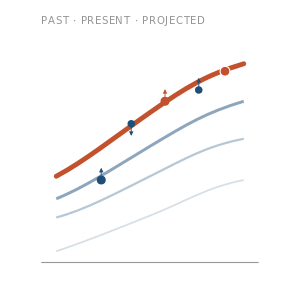
\includegraphics[height=6mm]{yc_logo.png}}
  \hfill{\ttfamily\scriptsize\color{ycmuted}yieldcartography.com/slides/snde/}
\end{frame}

\end{document}
